% Options for packages loaded elsewhere
\PassOptionsToPackage{unicode}{hyperref}
\PassOptionsToPackage{hyphens}{url}
%
\documentclass[
]{article}
\usepackage{lmodern}
\usepackage{amsmath}
\usepackage{ifxetex,ifluatex}
\ifnum 0\ifxetex 1\fi\ifluatex 1\fi=0 % if pdftex
  \usepackage[T1]{fontenc}
  \usepackage[utf8]{inputenc}
  \usepackage{textcomp} % provide euro and other symbols
  \usepackage{amssymb}
\else % if luatex or xetex
  \usepackage{unicode-math}
  \defaultfontfeatures{Scale=MatchLowercase}
  \defaultfontfeatures[\rmfamily]{Ligatures=TeX,Scale=1}
\fi
% Use upquote if available, for straight quotes in verbatim environments
\IfFileExists{upquote.sty}{\usepackage{upquote}}{}
\IfFileExists{microtype.sty}{% use microtype if available
  \usepackage[]{microtype}
  \UseMicrotypeSet[protrusion]{basicmath} % disable protrusion for tt fonts
}{}
\makeatletter
\@ifundefined{KOMAClassName}{% if non-KOMA class
  \IfFileExists{parskip.sty}{%
    \usepackage{parskip}
  }{% else
    \setlength{\parindent}{0pt}
    \setlength{\parskip}{6pt plus 2pt minus 1pt}}
}{% if KOMA class
  \KOMAoptions{parskip=half}}
\makeatother
\usepackage{xcolor}
\IfFileExists{xurl.sty}{\usepackage{xurl}}{} % add URL line breaks if available
\IfFileExists{bookmark.sty}{\usepackage{bookmark}}{\usepackage{hyperref}}
\hypersetup{
  pdftitle={Happy Valentines Day},
  pdfauthor={David M Vermillion},
  hidelinks,
  pdfcreator={LaTeX via pandoc}}
\urlstyle{same} % disable monospaced font for URLs
\usepackage[margin=1in]{geometry}
\usepackage{graphicx}
\makeatletter
\def\maxwidth{\ifdim\Gin@nat@width>\linewidth\linewidth\else\Gin@nat@width\fi}
\def\maxheight{\ifdim\Gin@nat@height>\textheight\textheight\else\Gin@nat@height\fi}
\makeatother
% Scale images if necessary, so that they will not overflow the page
% margins by default, and it is still possible to overwrite the defaults
% using explicit options in \includegraphics[width, height, ...]{}
\setkeys{Gin}{width=\maxwidth,height=\maxheight,keepaspectratio}
% Set default figure placement to htbp
\makeatletter
\def\fps@figure{htbp}
\makeatother
\setlength{\emergencystretch}{3em} % prevent overfull lines
\providecommand{\tightlist}{%
  \setlength{\itemsep}{0pt}\setlength{\parskip}{0pt}}
\setcounter{secnumdepth}{-\maxdimen} % remove section numbering
\ifluatex
  \usepackage{selnolig}  % disable illegal ligatures
\fi

\title{Happy Valentines Day}
\author{David M Vermillion}
\date{2/14/2021}

\begin{document}
\maketitle

\hypertarget{happy-valentines-day-my-beloved-shayla}{%
\subsubsection{Happy Valentines Day my beloved
Shayla!}\label{happy-valentines-day-my-beloved-shayla}}

\hypertarget{as-you-know-i-enjoy-dabbling-in-all-things-visualization-and-math.-i-figured-a-delightful-gift-for-you-would-be-to-create-a-little-card-telling-how-much-i-love-you-utilizing-some-mathiness.-i-used-one-of-my-graphing-programs-ggplot2-to-generate-the-message-shown-below-in-two-ways.}{%
\subsubsection{As you know, I enjoy dabbling in all things visualization
and math. I figured a delightful gift for you would be to create a
little card telling how much I love you, utilizing some mathiness. I
used one of my graphing programs (ggplot2) to generate the message shown
below in two
ways.}\label{as-you-know-i-enjoy-dabbling-in-all-things-visualization-and-math.-i-figured-a-delightful-gift-for-you-would-be-to-create-a-little-card-telling-how-much-i-love-you-utilizing-some-mathiness.-i-used-one-of-my-graphing-programs-ggplot2-to-generate-the-message-shown-below-in-two-ways.}}


\includegraphics[width=0.3\linewidth]{I}

\includegraphics[width=0.3\linewidth]{Heart2}

\includegraphics[width=0.3\linewidth]{U}

\begin{center}\rule{0.5\linewidth}{0.5pt}\end{center}

\begin{center}
\includegraphics[width=0.5\linewidth]{I} \end{center}

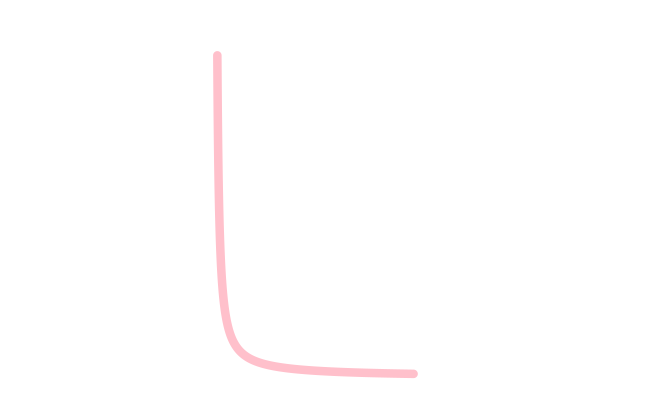
\includegraphics[width=0.25\linewidth]{L}

\includegraphics[width=0.25\linewidth]{O}

\includegraphics[width=0.25\linewidth]{V}

\includegraphics[width=0.25\linewidth]{E}

\begin{center}
\includegraphics[width=0.5\linewidth]{U} \end{center}

\hypertarget{i-also-wanted-to-show-you-another-heart-i-created-to-express-my-love.}{%
\subsubsection{I also wanted to show you another heart I created to
express my
love.}\label{i-also-wanted-to-show-you-another-heart-i-created-to-express-my-love.}}


\includegraphics[width=0.5\linewidth]{Heart1}

\hypertarget{these-are-the-equations-i-used-to-make-the-letters-and-the-hearts-with-the-exception-of-the-i-and-o-which-i-created-using-graph-code.}{%
\subsubsection{These are the equations I used to make the letters and
the hearts, with the exception of the I and O, which I created using
graph
code.}\label{these-are-the-equations-i-used-to-make-the-letters-and-the-hearts-with-the-exception-of-the-i-and-o-which-i-created-using-graph-code.}}

\(\LARGE y = \frac{1}{x} \hspace{1cm}\)

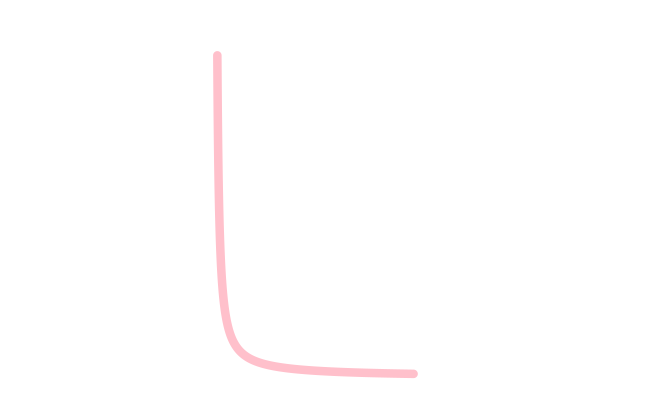
\includegraphics[width=0.5\linewidth]{L}

\(\LARGE y=\lvert x\rvert \hspace{3cm}\)


\includegraphics[width=0.5\linewidth]{V}

\(\LARGE x=-3\lvert sin(y)\rvert \hspace{6cm}\)


\includegraphics[width=0.5\linewidth]{E}

\(\begin{align} & \LARGE x=4(3sin(\theta) - sin(3\theta))\\ &\LARGE y=13cos(\theta) - 5cos(2\theta) - cos(4\theta) \end{align}\)


\includegraphics[width=0.5\linewidth]{Heart1}

\(\LARGE r(\theta) = 2-2sin\theta+sin\theta \frac{\sqrt{\lvert cos\theta \rvert}}{sin\theta + 1.4} \hspace{1.2cm}\)


\includegraphics[width=0.5\linewidth]{Heart2}

\hypertarget{with-love-from-your-adoring-husband}{%
\section{With love from your adoring
husband,}\label{with-love-from-your-adoring-husband}}

\hypertarget{david}{%
\section{David}\label{david}}

\end{document}
